
\section{Geometron in 3d and Beyond}


\subsection{Structure, Definitions and Formats}

\begin{figure}
	\centering
	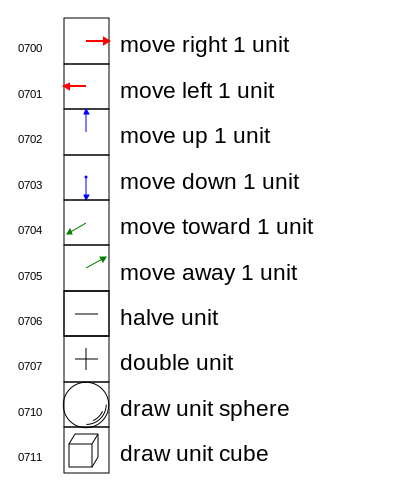
\includegraphics[width=4in]{figures/geometron3d/actions.png}
	\caption[actions3d]
	{Actions.}
\end{figure}

Whimsy Castle

\begin{figure}
	\centering
	\includegraphics[width=4in]{figures/geometron3d/whimsycastle.png}
	\caption[whimsycastle]
	{castle 3d.}
\end{figure}


\begin{figure}
	\centering
	\includegraphics[width=4in]{figures/geometron3d/whimsycastleturret.png}
	\caption[whimsycastleturret]
	{Turret construction.}
\end{figure}

\begin{figure}
	\centering
	\includegraphics[width=4in]{figures/geometron3d/whimsycastlespelling.png}
	\caption[whimsycastlespelling]
	{whimsycastlespelling.}
\end{figure}


\begin{figure}
	\centering
	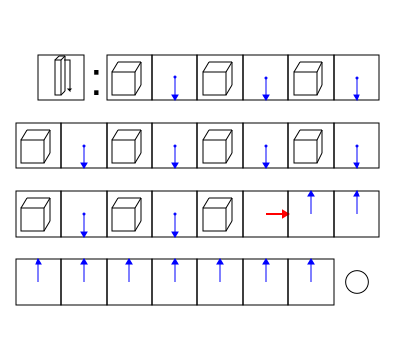
\includegraphics[width=4in]{figures/geometron3d/shapebuilding1.png}
	\caption[shapebuilding1]
	{shapebuilding1.}
\end{figure}

\begin{figure}
	\centering
	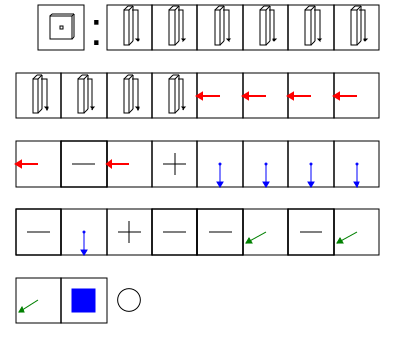
\includegraphics[width=4in]{figures/geometron3d/shapebuilding2.png}
	\caption[shapebuilding2]
	{shapebuilding2.}
\end{figure}

\subsection{Icons and Trash Robot}


\begin{figure}
	\centering
	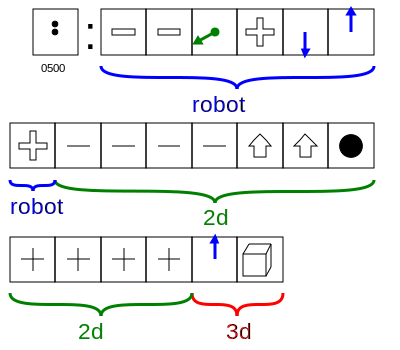
\includegraphics[width=4in]{figures/geometron3d/robot0500.png}
	\caption[robot0500]
	{robot0500.}
\end{figure}

\begin{figure}
	\centering
	\includegraphics[width=4in]{figures/geometron3d/trashrobot3d.png}
	\caption[trashrobot3d]
	{trashrobot3d.}
\end{figure}

\subsection{Rotations and Higher Dimensions}



\begin{figure}
	\centering
	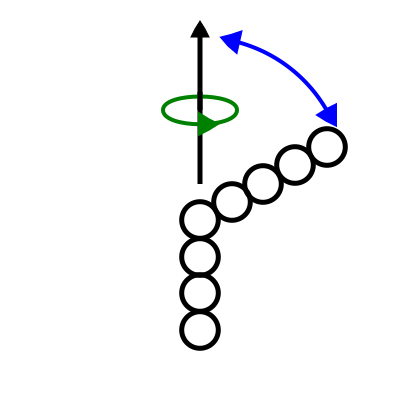
\includegraphics[width=4in]{figures/geometron3d/angles.png}
	\caption[angles]
	{angles.}
\end{figure}

\subsection{Virtual and Augmented Reality, the 3d Web and Games}

\begin{itemize}
\tightlist
\item
  where it exists in hypercube, concepts of movement and construction, cursor
\item
  file formats and software: THREEjs, .x3d, how they are used, 3d printing
\item
  fonts: examples of pixel font of standard English letters and braille with hemispheres
\item
  rotation angles of many part robotic arm tools
\item
  quantum geometron: rotations in hilbert space, representation of hypercube in state of quantum processor, direct mapping to protein folding without gates 
\item
  writing 3d geometron apps, how to use, how to expand and rewrite
\item 
  detailed documentation of the code
\end{itemize}